\documentclass[main.tex]{subfiles}
\begin{document}
    
    \subsection{Car Increment Simulation}
        Le simulazioni mostrano che fissata la città, l'indice di traffico aumenta all'aumentare delle automobili
        e tende a 1 per il numero di automobili che tende a zero. Ovviamente tale simulazione non avrebbe senso, per ciò 
        partiamo da almeno 1 macchina nella città, l'indice di traffico che emerge dalla simulazione con una sola macchina
        sarà 1 poiché non può esistere un rallentamento.
        In Fig. \ref{fig:3} è riportato l'esito di circa 70 simulazioni che incrementano di 1 il numero di automobili da 1 a 2000.
        Ciò è stato fatto su una città $5 \times 5$ senza sensi unici per verificare che effettivamente il traffico aumentasse
        all'aumentare delle auto.

        \begin{figure}[H]
            \begin{minipage}{.5\textwidth}
                \centering
                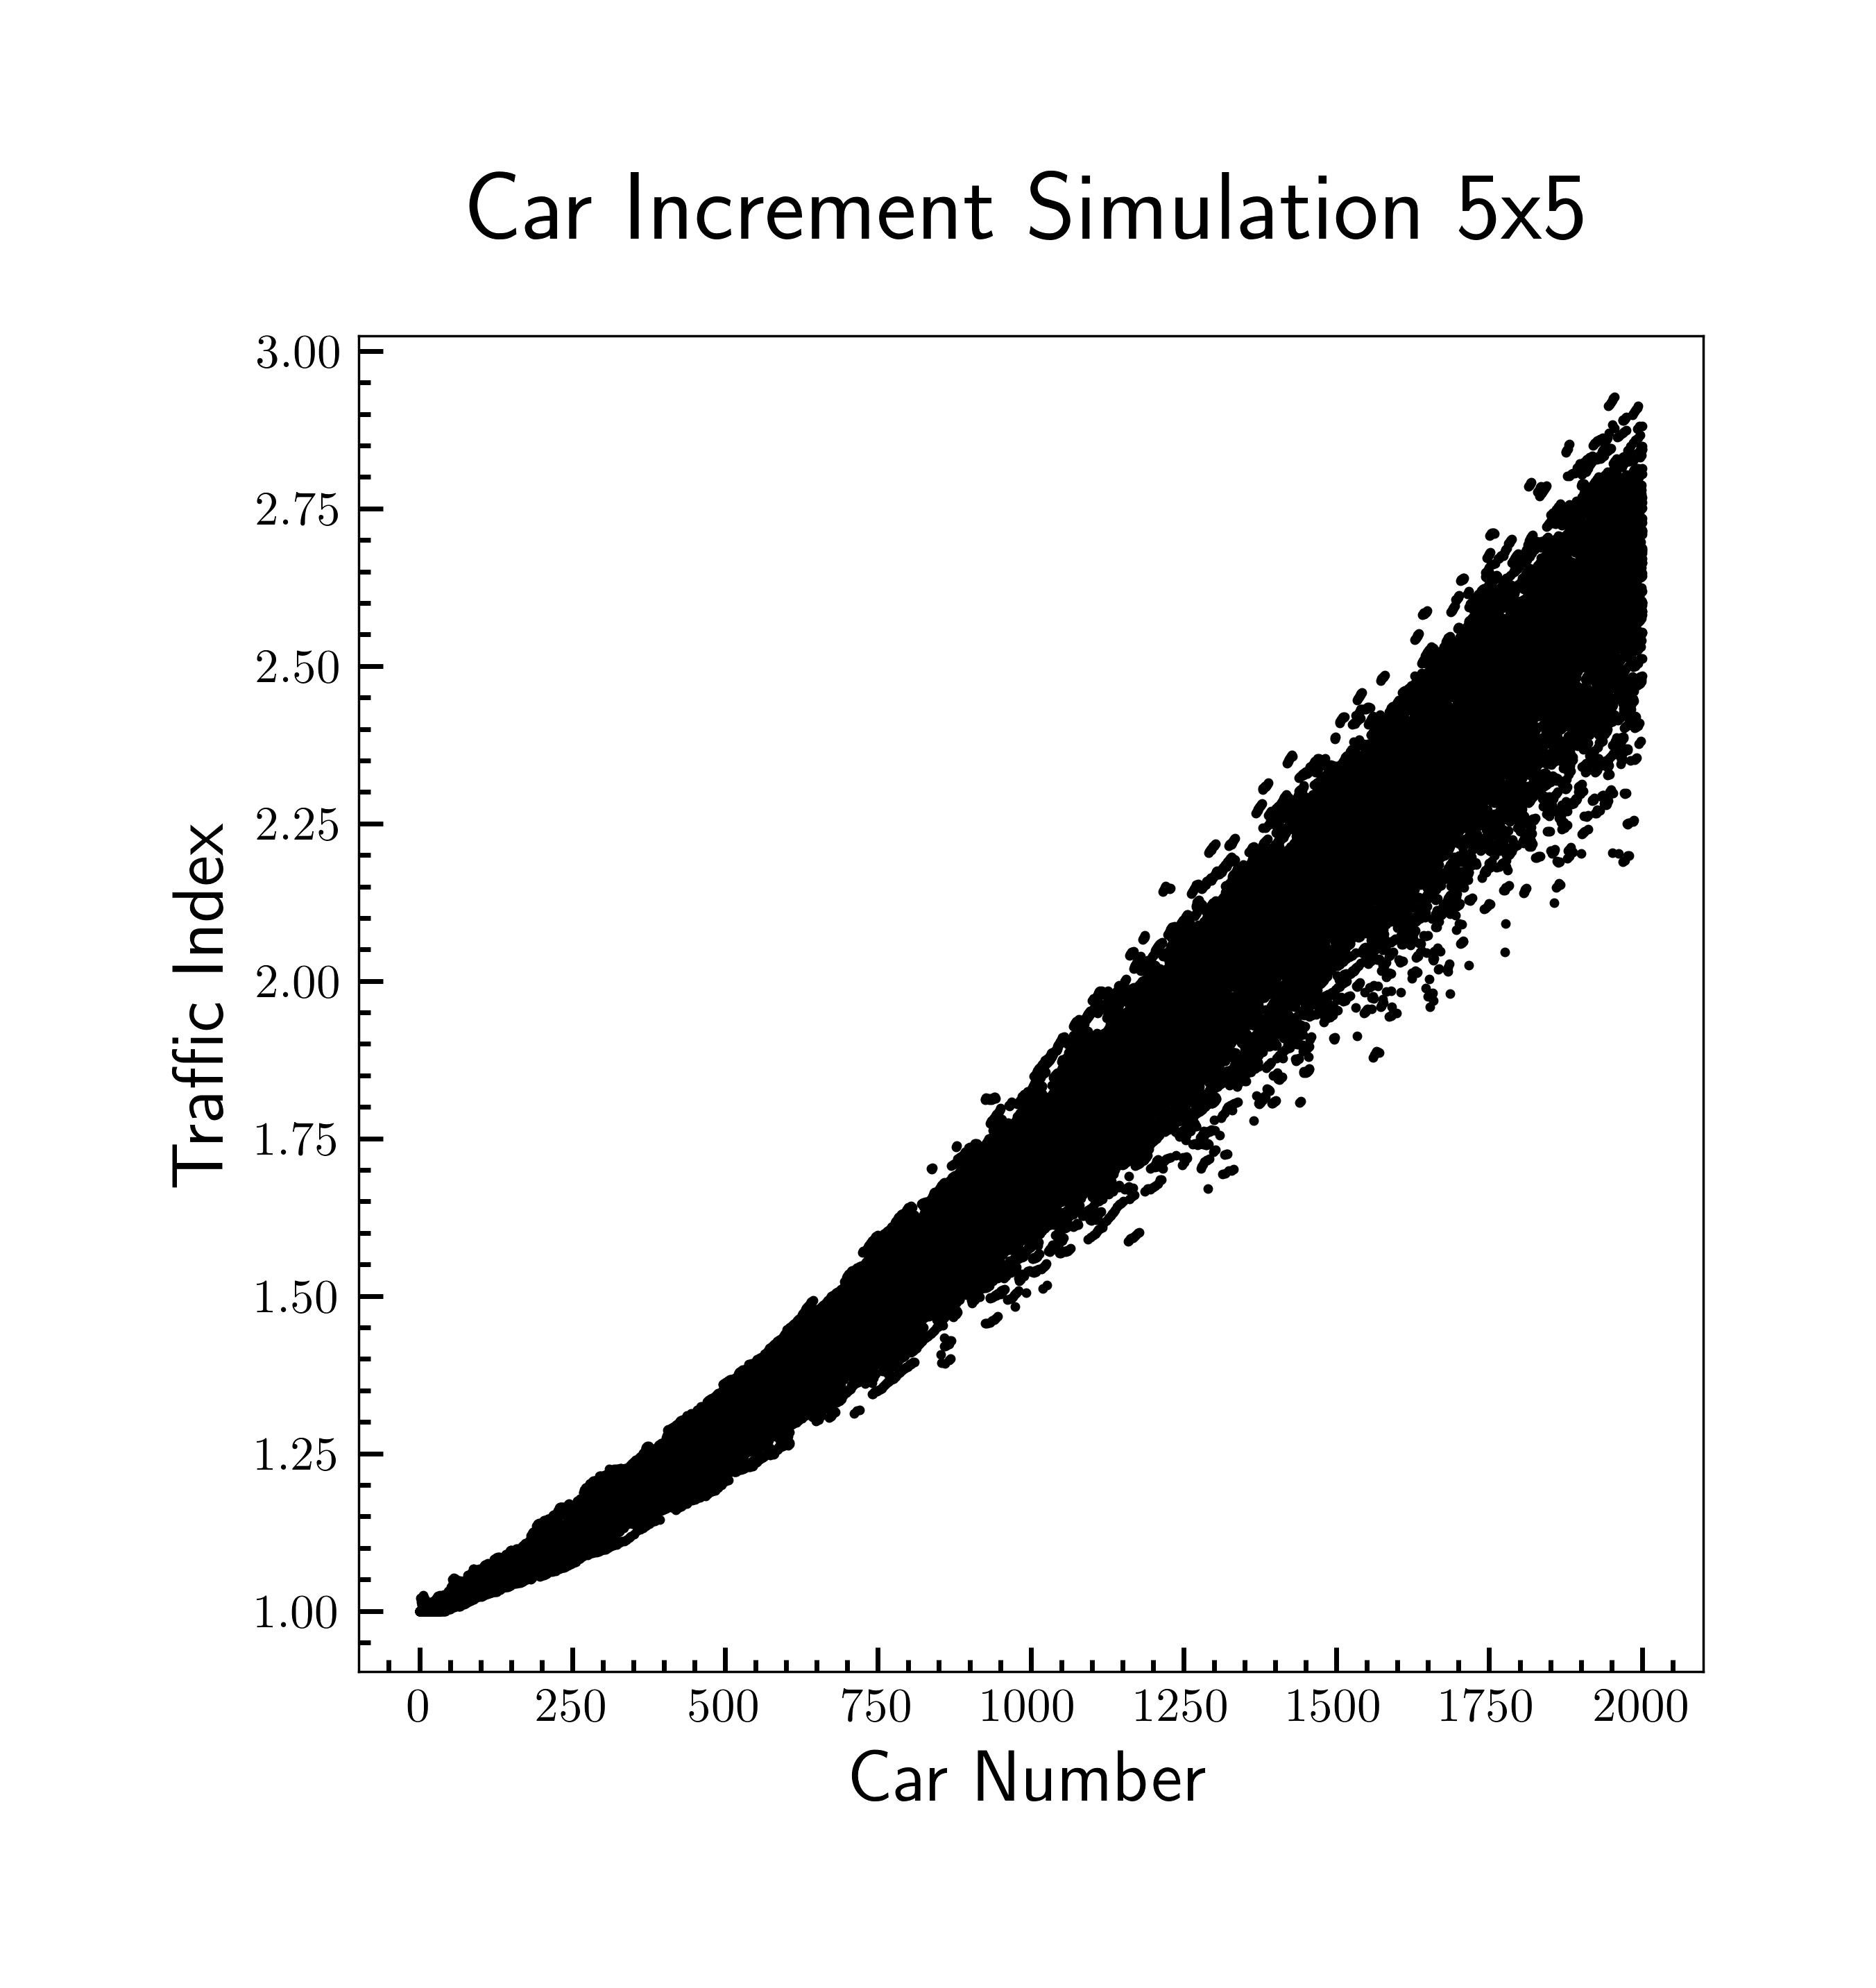
\includegraphics[width=8cm, height=8cm]{car_increment5x5.png}
                \caption{Car Increment Simulation\\ su una città $5 \times 5$ senza sensi unici.}
                \label{fig:3}
            \end{minipage}
            \begin{minipage}{.5\textwidth}
                \centering
                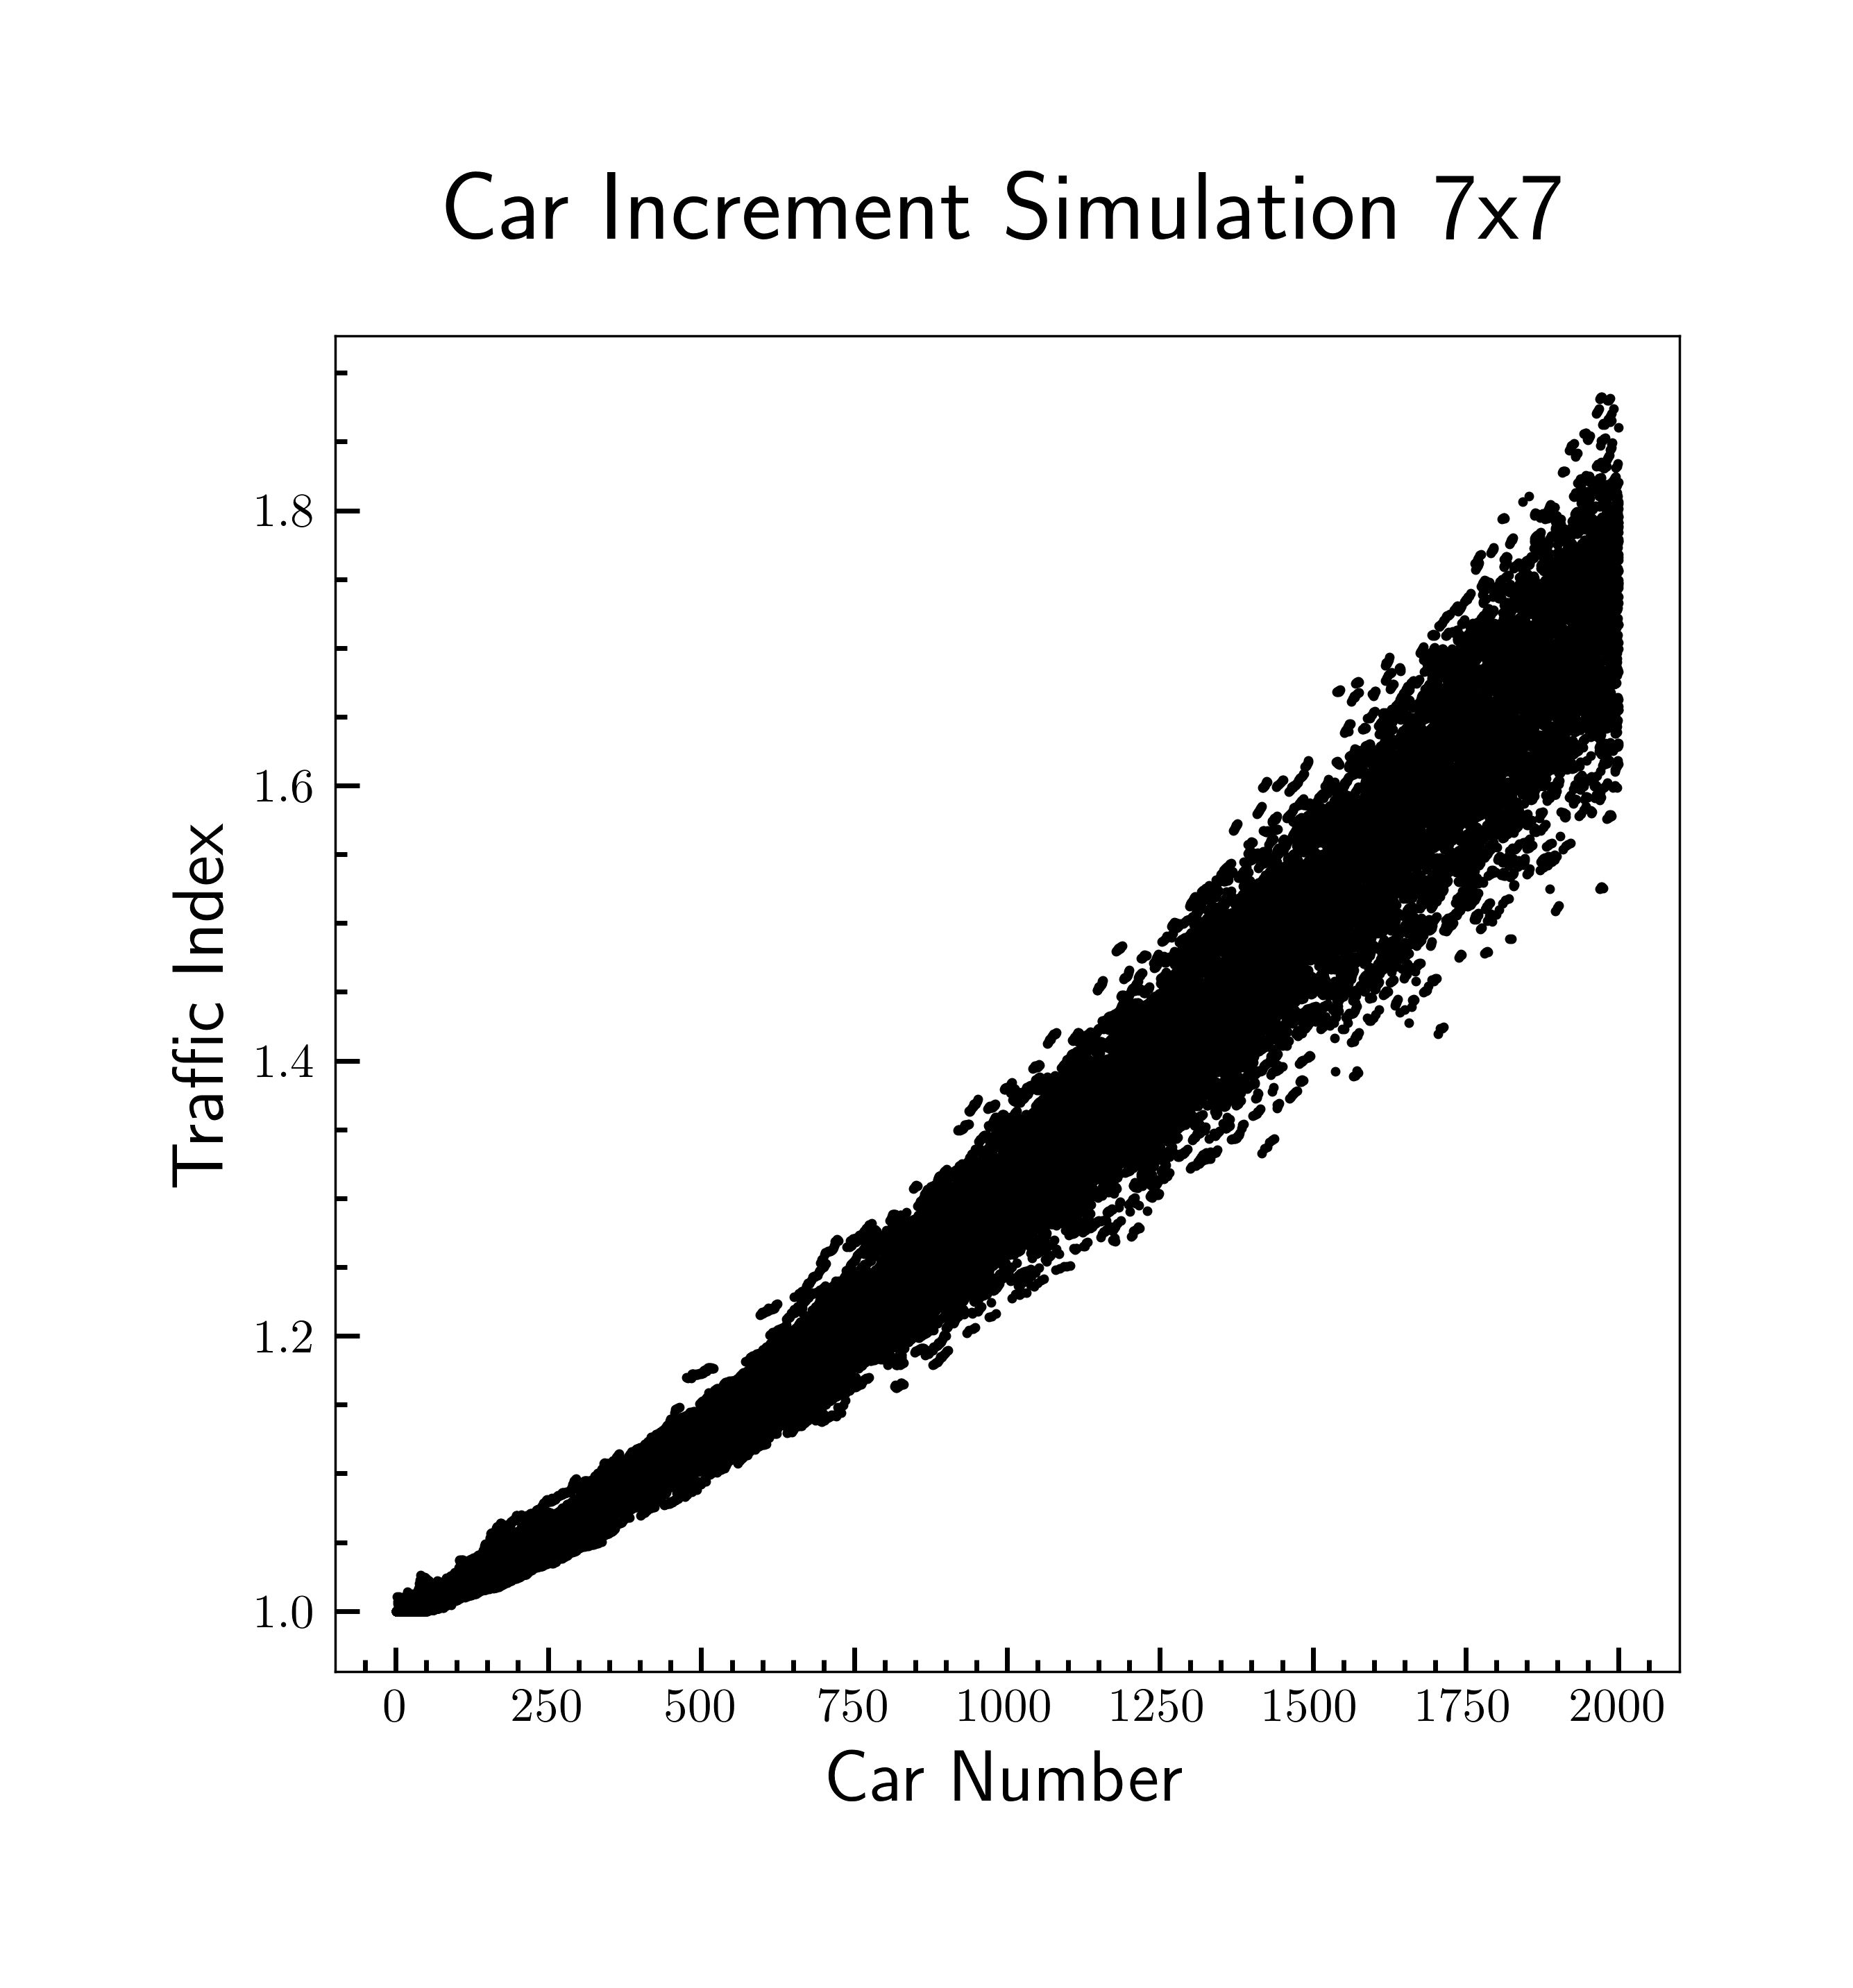
\includegraphics[width=8cm, height=8cm]{car_increment7x7.png}
                \caption{Car Increment Simulation su una città $7 \times 7$ senza sensi unici.}
                \label{fig:4}
            \end{minipage}
        \end{figure}

        Per entrambe queste simulazioni si è usata la seguente statistica delle strade:
        \begin{itemize}
            \item media della lunghezza : 20
            \item deviazione standard della lunghezza : 10
            \item lunghezza massima : 30
            \item lunghezza minima : 10
        \end{itemize}

        Un' osservazione interessante che può essere fatta a partire da queste statistiche è che su città rispettivamente
        $5 \times 5$ e $7 \times 7$ generano una superficie stradale media data da $20 \times 5 \times 4 \times 2 = 800$ e
        $20 \times 7 \times 6 \times 2 = 1680$. Data questa considerazione, notiamo che quando il numero di auto è confrontabile con 
        la superficie media nelle due simulazioni l'indice di traffico si trova sempre attorno a 1.5.
        Perciò possiamo pensare che senza ulteriori modifiche topologiche, l'indice di traffico su una città a griglia
        senza sensi unici dipenda esclusivamente dalla densità di automobili.

        Il fatto che a densità uguale a 1 il programma non si blocchi è dovuto ad un controllo che fa partire le auto con diversi ritardi,
        quindi non tutte le auto indicate da car number saranno nella città contemporaneamente.
        Da questa anilisi preliminare possiamo concludere che il traffico emerge dal nostro modello e dipende dalla densità di auto,
        come suggerito da tutti i modelli di traffico esistenti.

    \subsection{Oneway Increment Simulation}
        Per vedere se aumentare il numero di sensi unici è in alcuni casi conveniente, abbiamo fatto una simulazione aumentando la frazione di sensi unici 
        fissate 1000 automobili utilizzando le stesse statistiche stradali della sezione precedente. Tale simulazione è stata eseguita per diverse larghezze dei sensi unici, ovvero una, due e tre corsie.
        L'incremento del parametro di generazione \_oneway\_fraction è stato scelto essere 0.001.
        In Fig. \ref{fig:5} è mostrata la simulazione con sesi unici larghi una sola corsia che, causando una riduzione della superficie media, è chiaramente sconveniente.

        \begin{figure}[H]
            \centering
            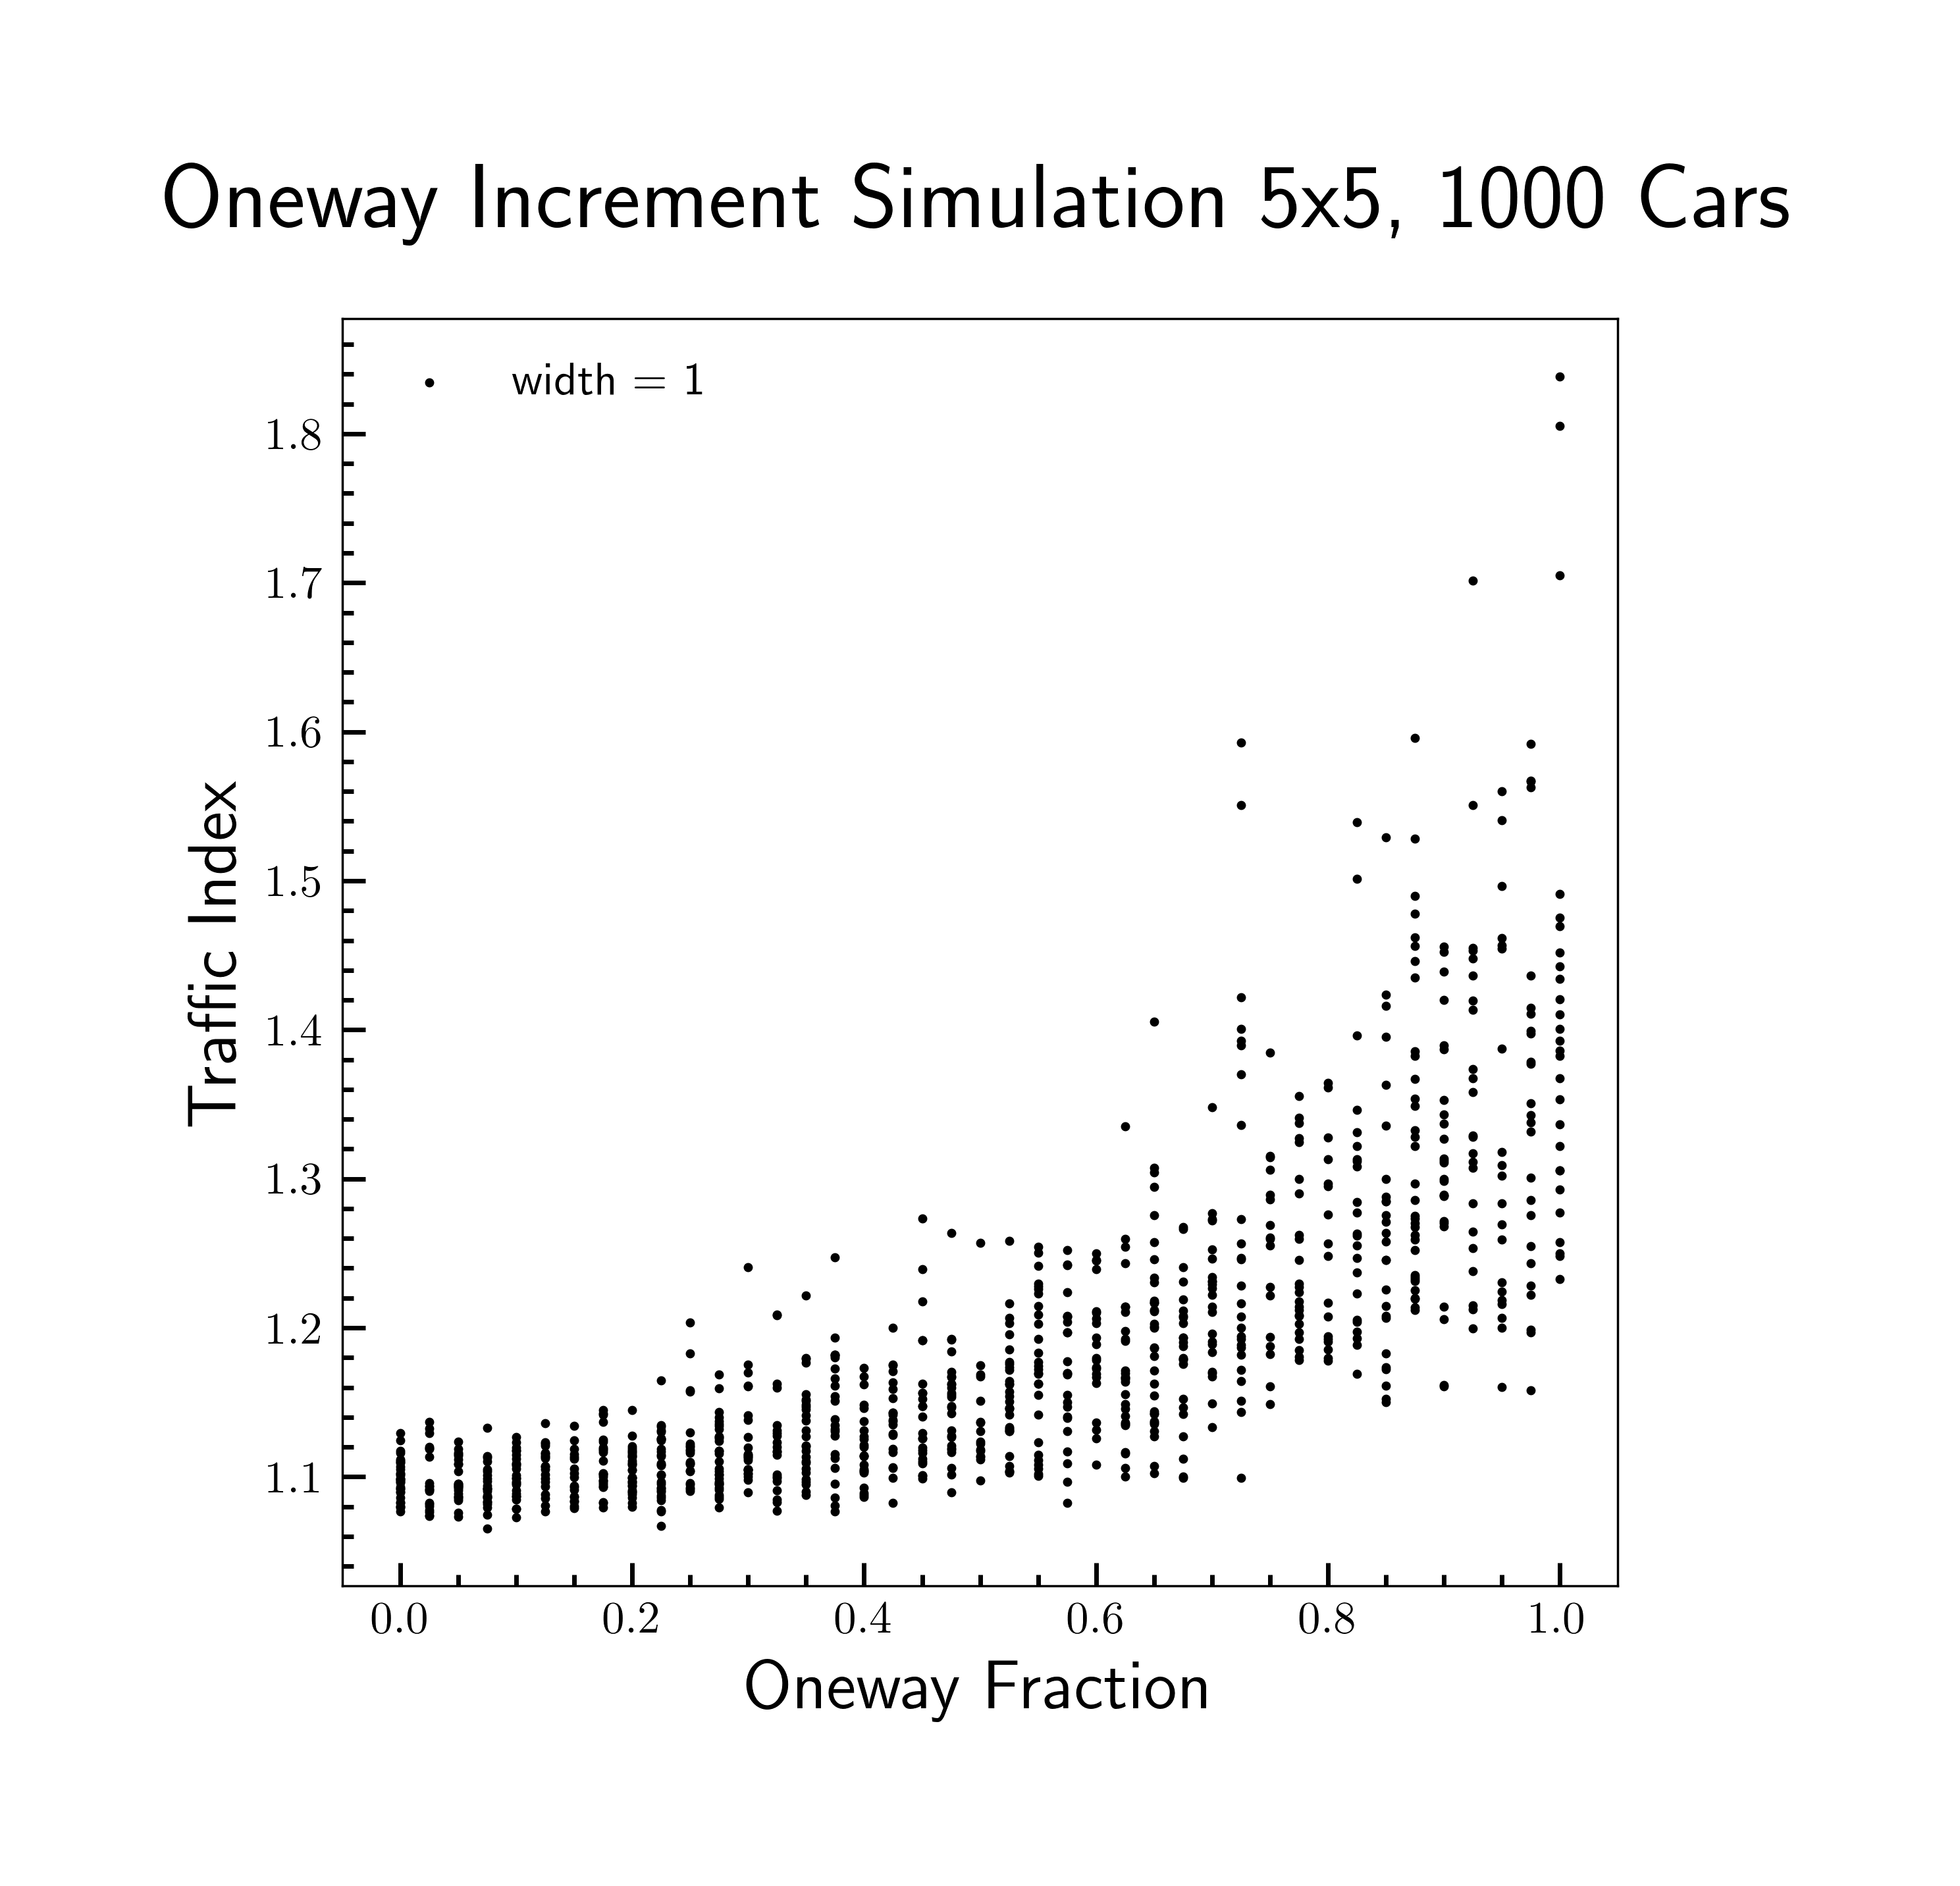
\includegraphics[width=10cm, height=10cm]{oneway_increment_1.png}  
            \caption{Oneway Increment Simulation su una città $5 \times 5$, con larghezza uguale a uno.}
            \label{fig:5}
        \end{figure}

        Da questo grafico possiamo notare che il traffico aumenterà sempre aumentando i sensi unici a meno della fluttuazione dovuta
        al posizionamento dei sensi unici nella città. Infatti si può notare che la sezione verticale della fascia nera del grafico si allarga
        andando verso destra. Ciò significa che in città con tanti sensi unici l'indice di traffico dipenderà molto dal modo in cui essi sono disposti
        e non solo dalla frazione.

        \newpage

        In Fig. \ref{fig:6} e in Fig. \ref{fig:7} è mostrata la stessa simulazione con sensi unici rispettivamente a due e tre corsie.

        \begin{figure}[H]
            \begin{minipage}{.5\textwidth}
                \centering
                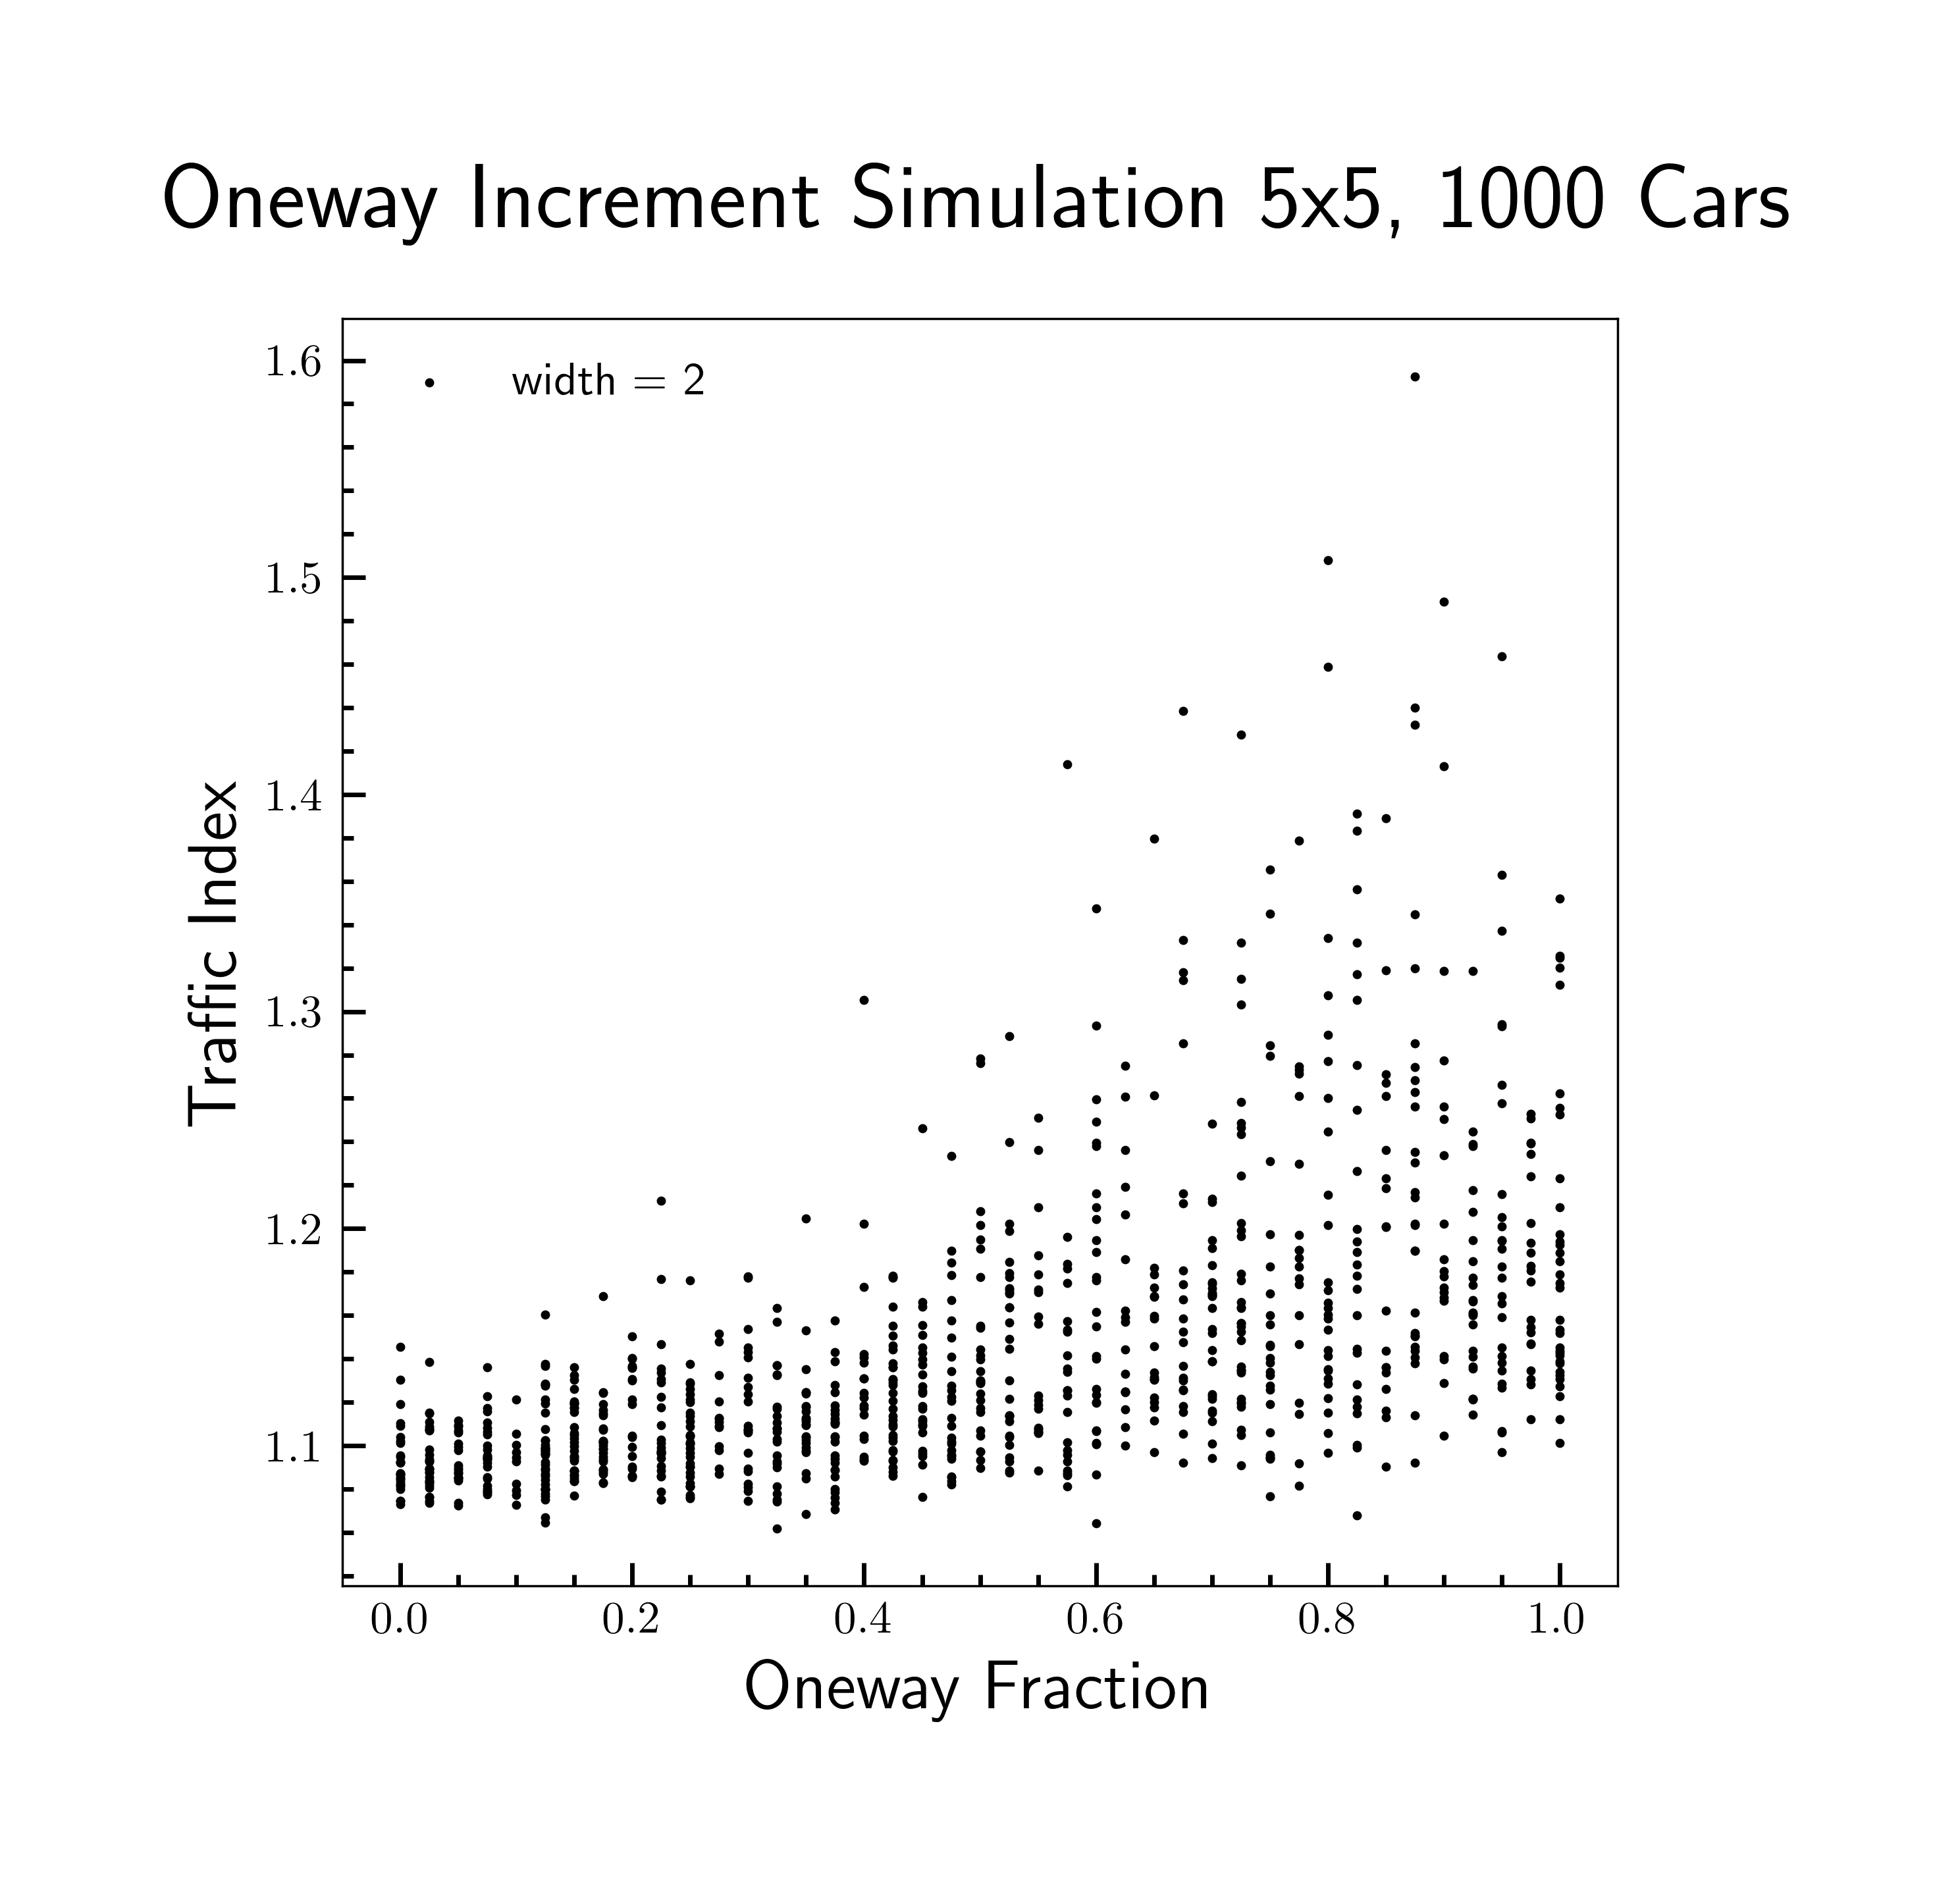
\includegraphics[width=8cm, height=8cm]{oneway_increment_2.png}  
                \caption{Oneway Increment Simulation su\\ una città $5 \times 5$, con larghezza uguale a due.}
                \label{fig:6}
            \end{minipage}
            \begin{minipage}{.5\textwidth}
                \centering
                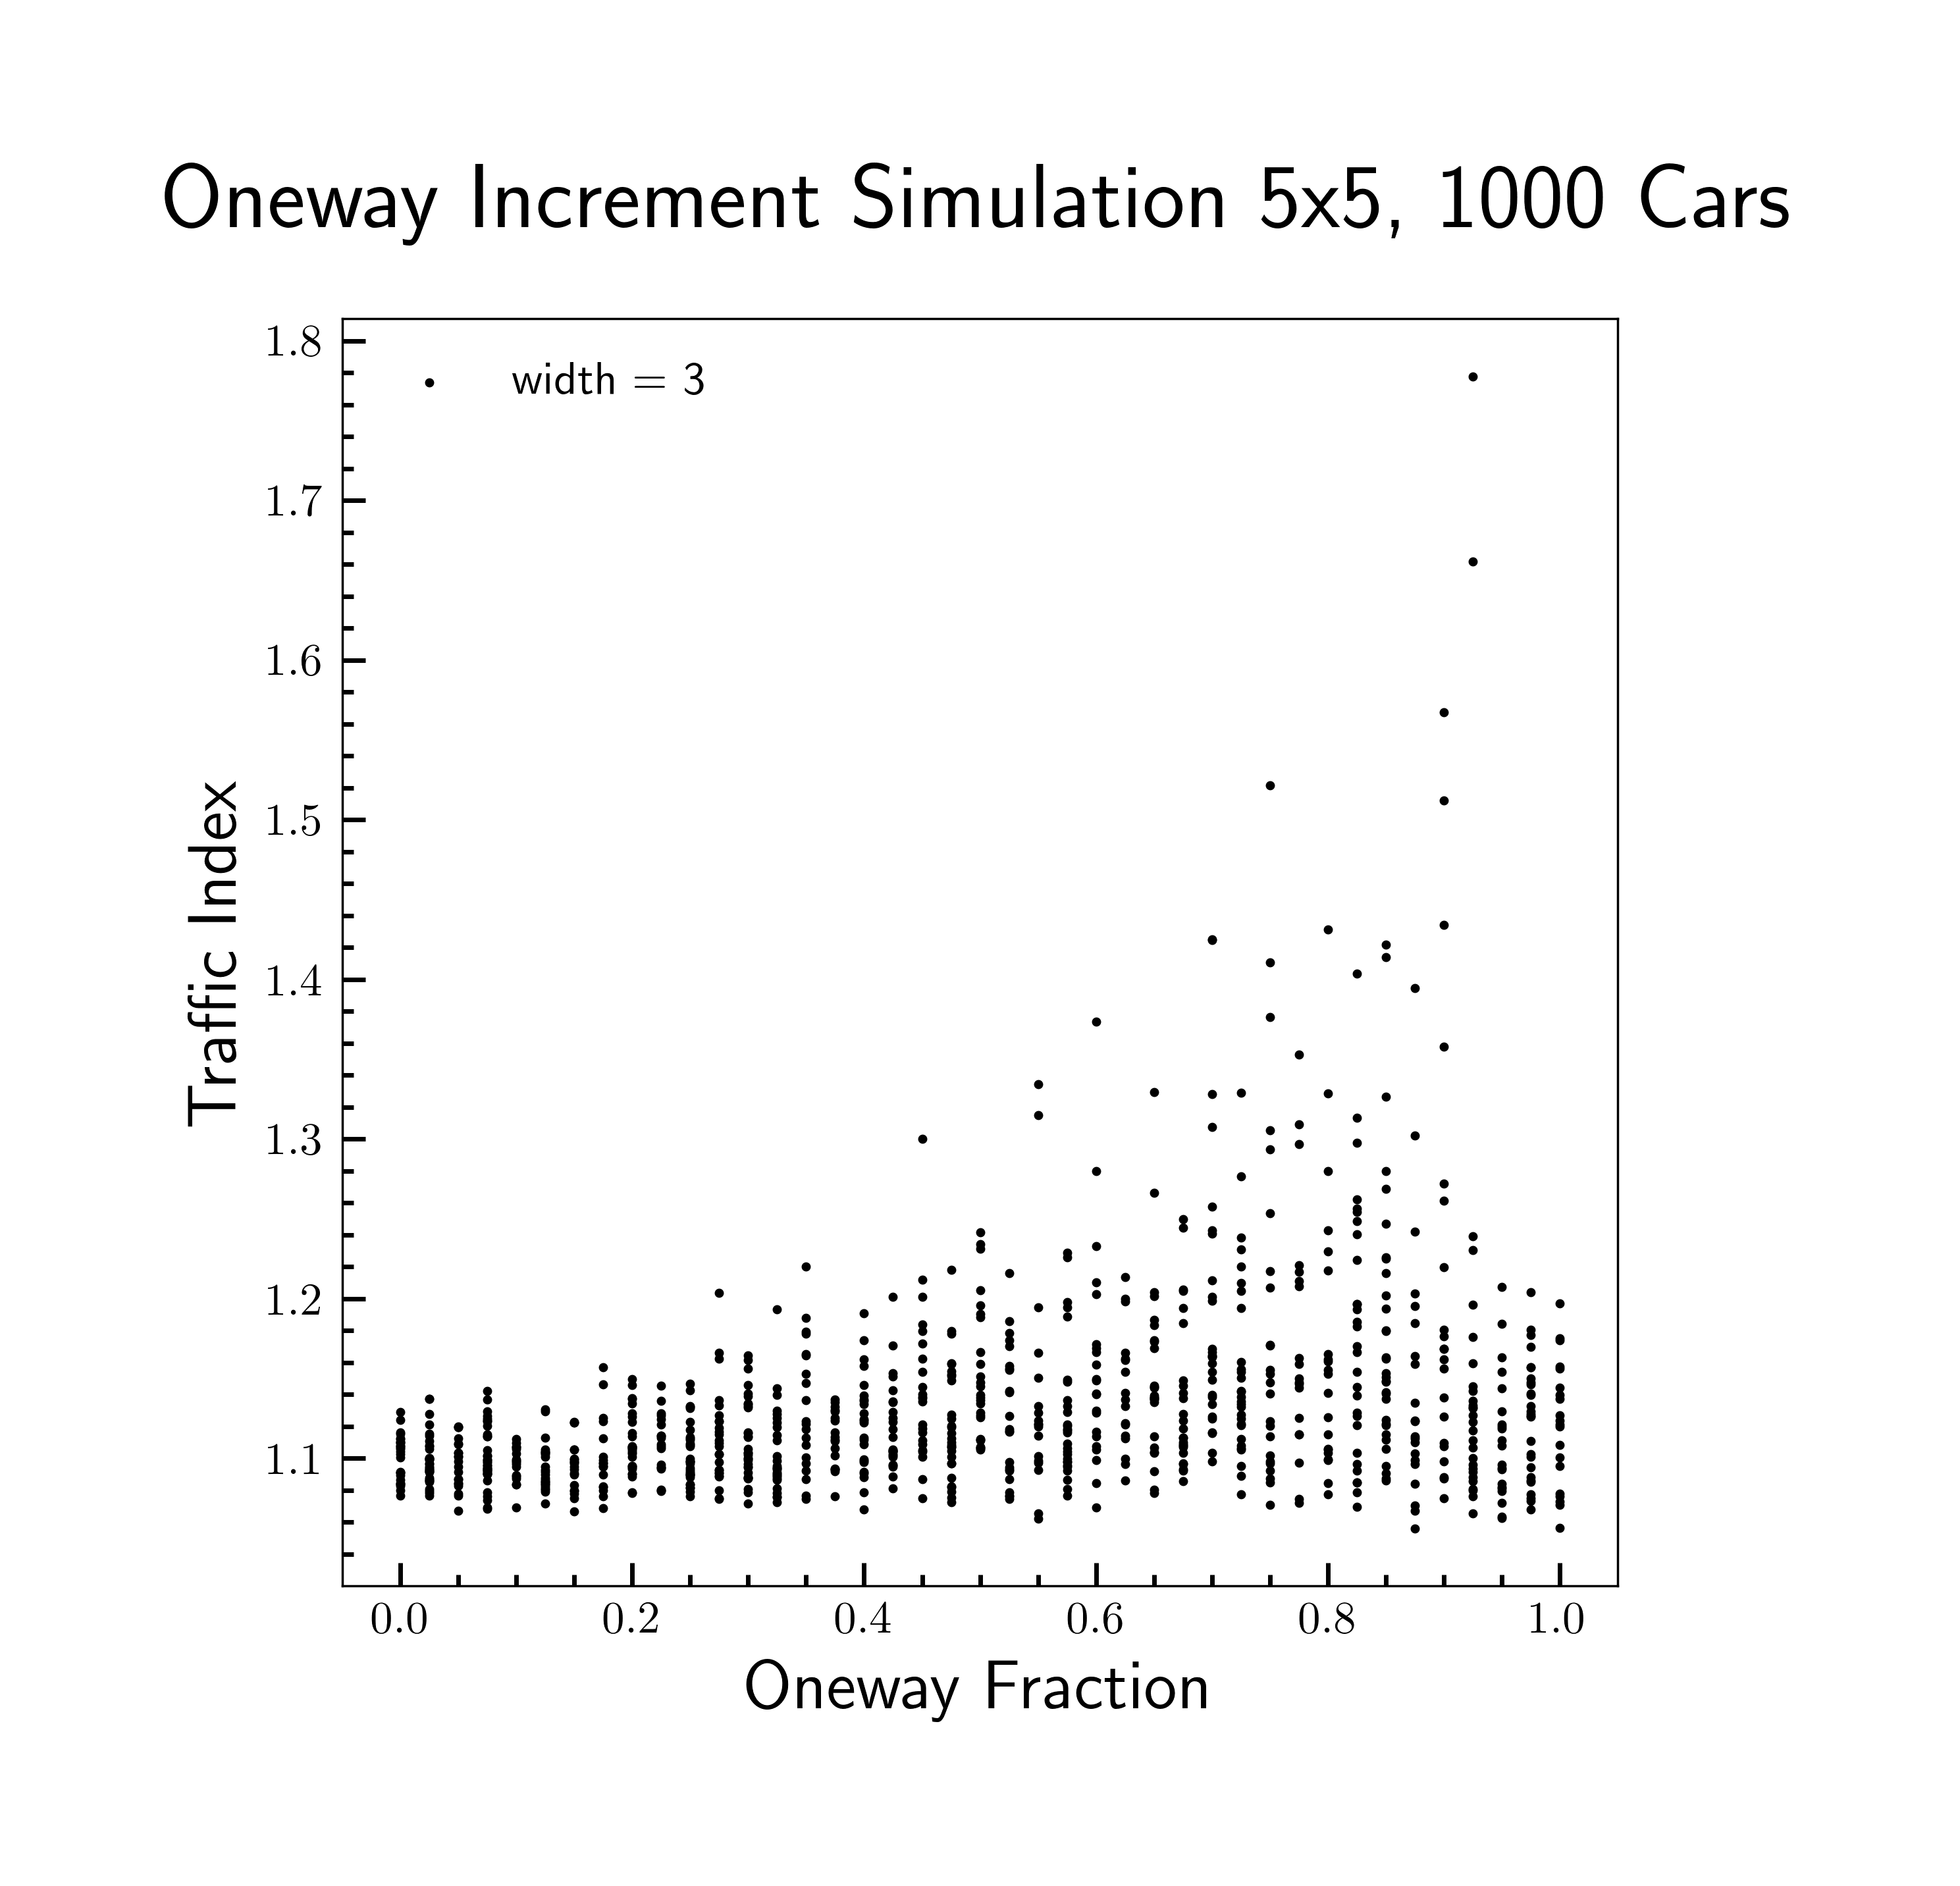
\includegraphics[width=8cm, height=8cm]{oneway_increment_3.png}  
                \caption{Oneway Increment Simulation su una città $5 \times 5$, con larghezza uguale a tre.}
                \label{fig:7}
            \end{minipage}
        \end{figure}

        In Fig. \ref{fig:6} a differenza del grafico precedente, notiamo che per un'alta frazione di sensi unici si hanno comunque città
        con un indice di traffico relativamente basso. Quindi possiamo dire che esiste un modo per disporre molti sensi unici a molte corsie per
        ridurre l'indice di traffico. Tuttavia tale fatto potrebbe anche essere dovuto all'aumento della superficie media della città all'aumentare dei 
        sensi unici, che perciò andrebbe a ridurre la densità di automobili riducendo l'indice di traffico.
        Tale effetto è maggiormente accentuato in Fig. \ref{fig:7}, mettendo sensi unici a tre corsie.\\
        \hfill\\

        In questi tre grafici l'effetto di "quantizzazione" della frazione di sensi unici è dovuto alle piccole dimensioni della città.
        Infatti il numero ridotto di strade, questa volta intese senza direzione, fa in modo che le frazioni di sensi unici non possano variare
        continuamente.

        \newpage

        Un'altra analisi che è stata fatta, approssimando linearmente gli esiti delle car increment simulation a diverse frazioni di sensi unici, consiste nel vedere
        come la pendenza di tali rette varia al variare dei sensi unici, il grafico è riportato in Fig. \ref{fig:8} mentre in Fig. \ref{fig:9} è riportata 
        una giustificazione grafica dell'approssimazione lineare. La pendenza di tali rette rappresenta la risposta della città all'aumentare della densità di 
        automobili.

        \begin{figure}[H]
            \begin{minipage}{.5\textwidth}
                \centering
                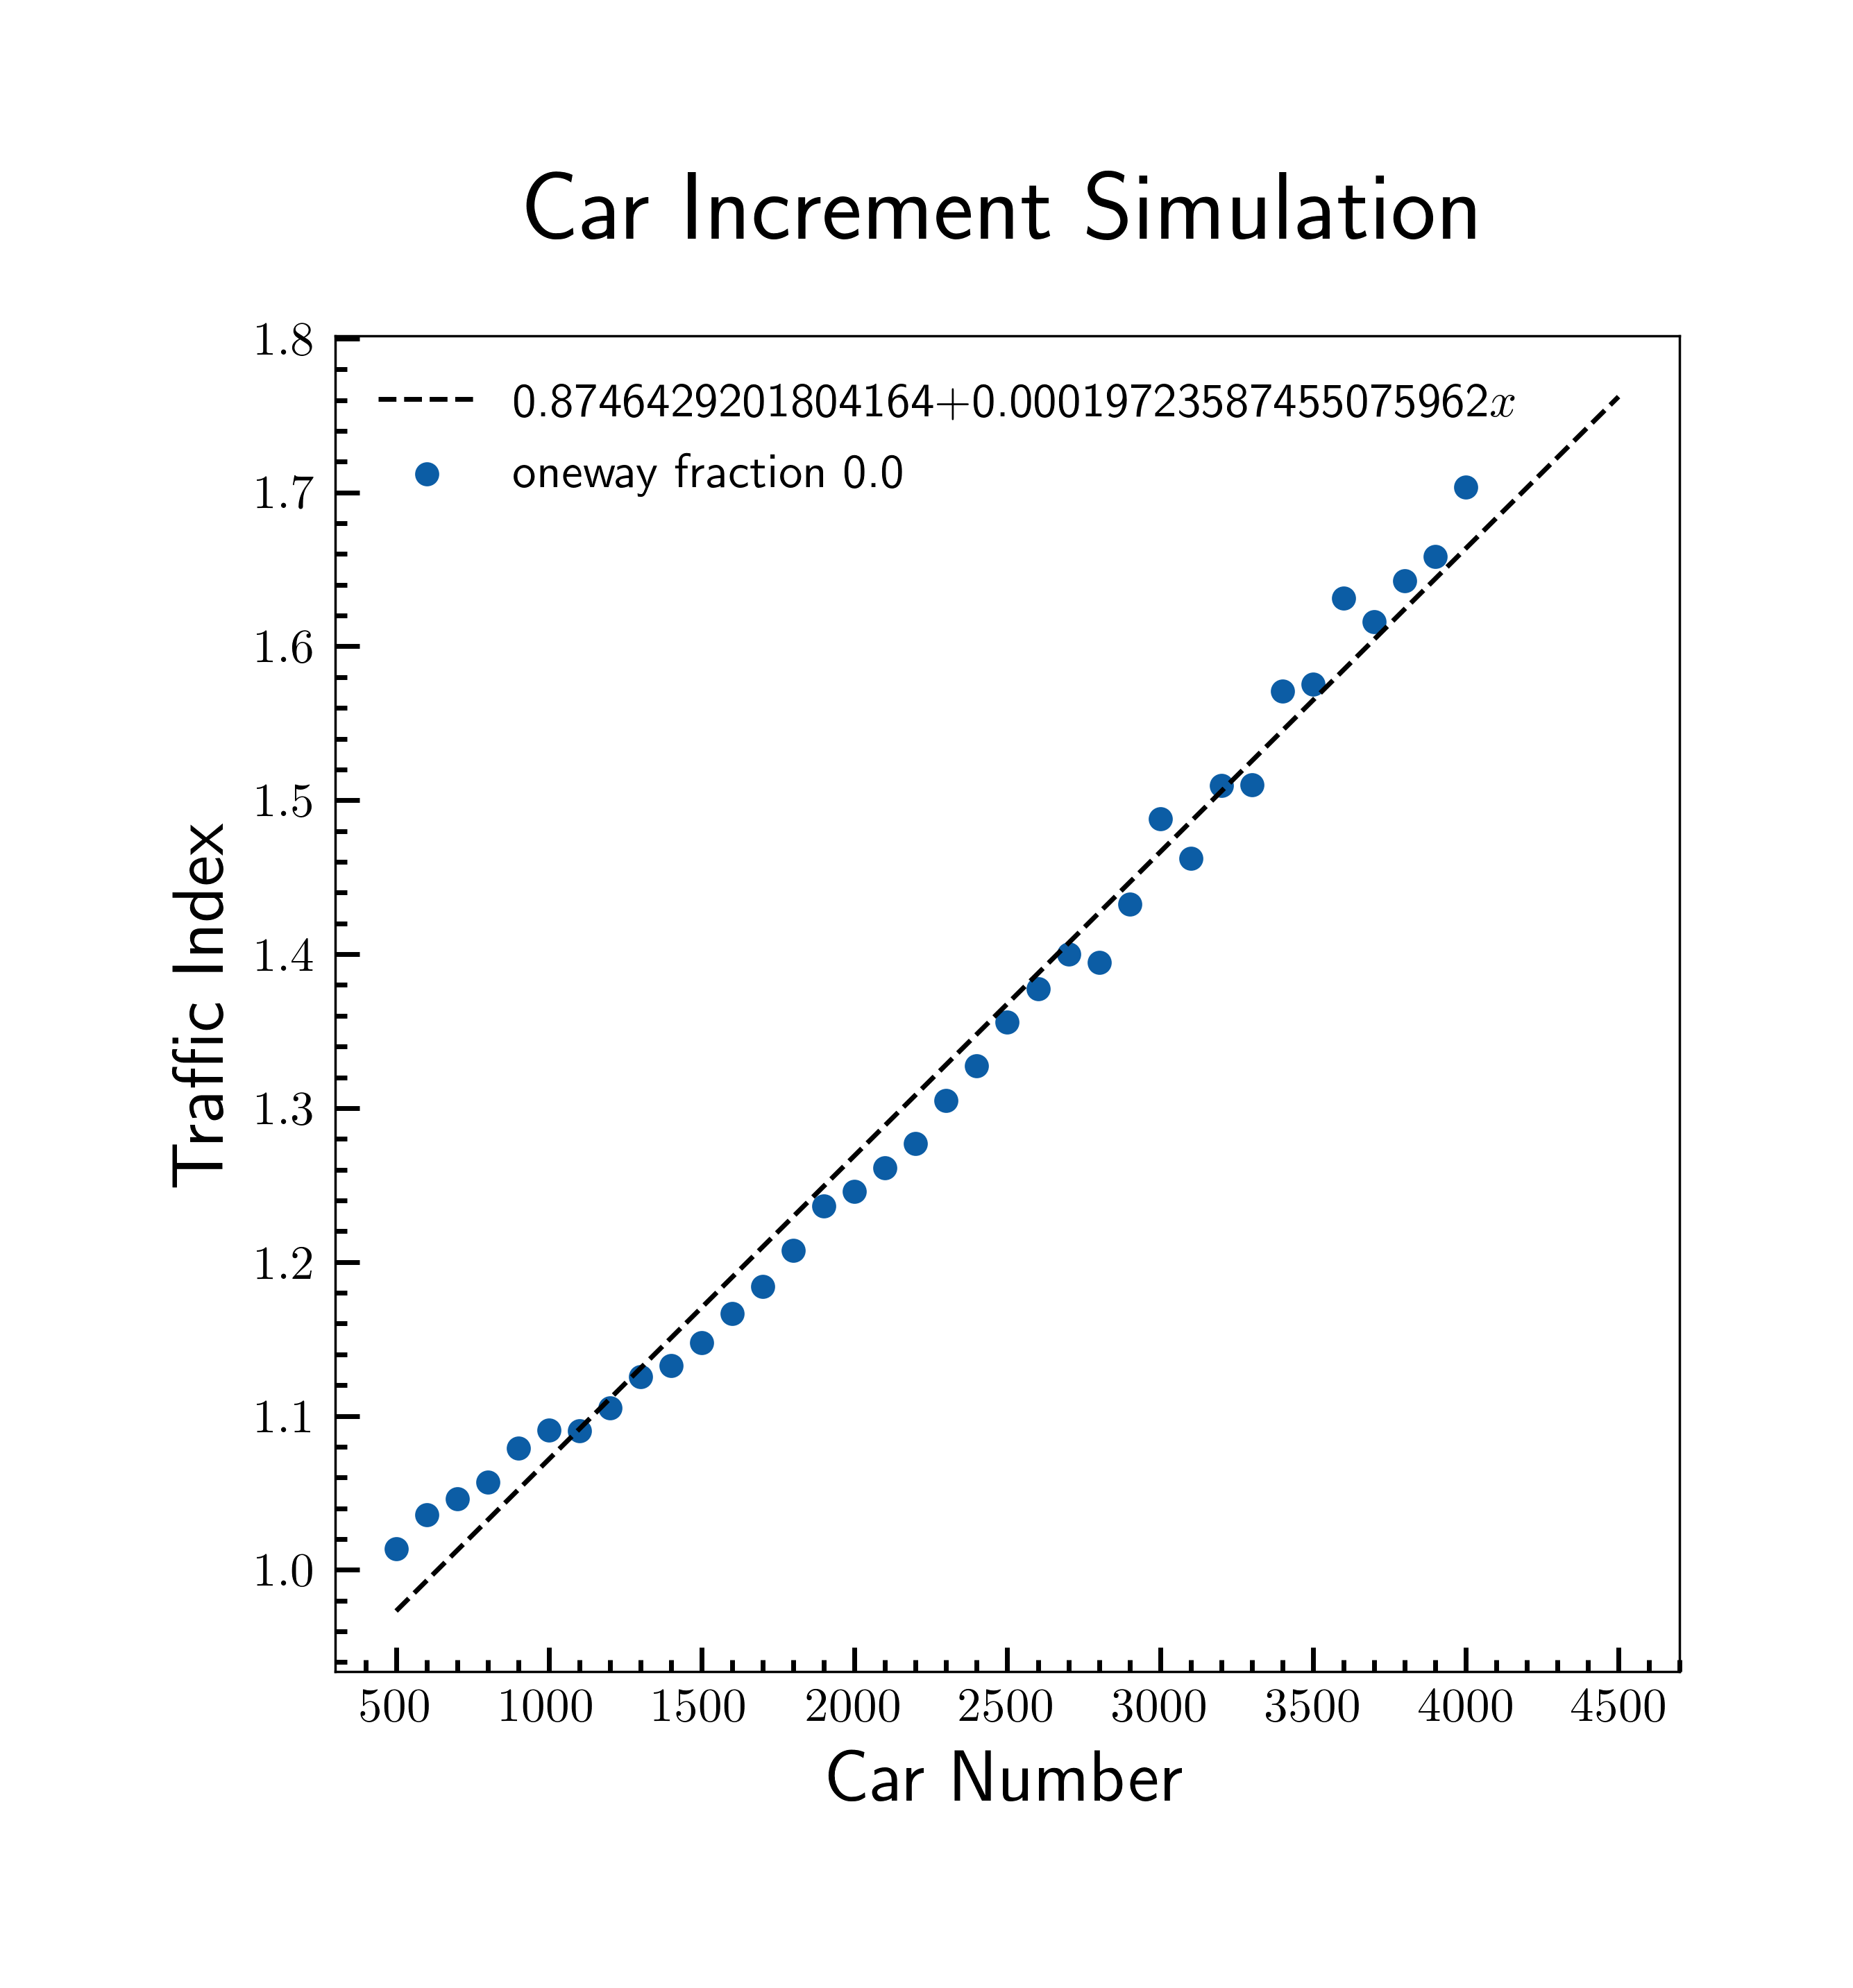
\includegraphics[width=8cm, height=8cm]{car_increment.png}
                \caption{Car Increment Simulation su\\ una città $10 \times 10$.}
                \label{fig:9}
            \end{minipage}
            \begin{minipage}{.5\textwidth}
                \centering
                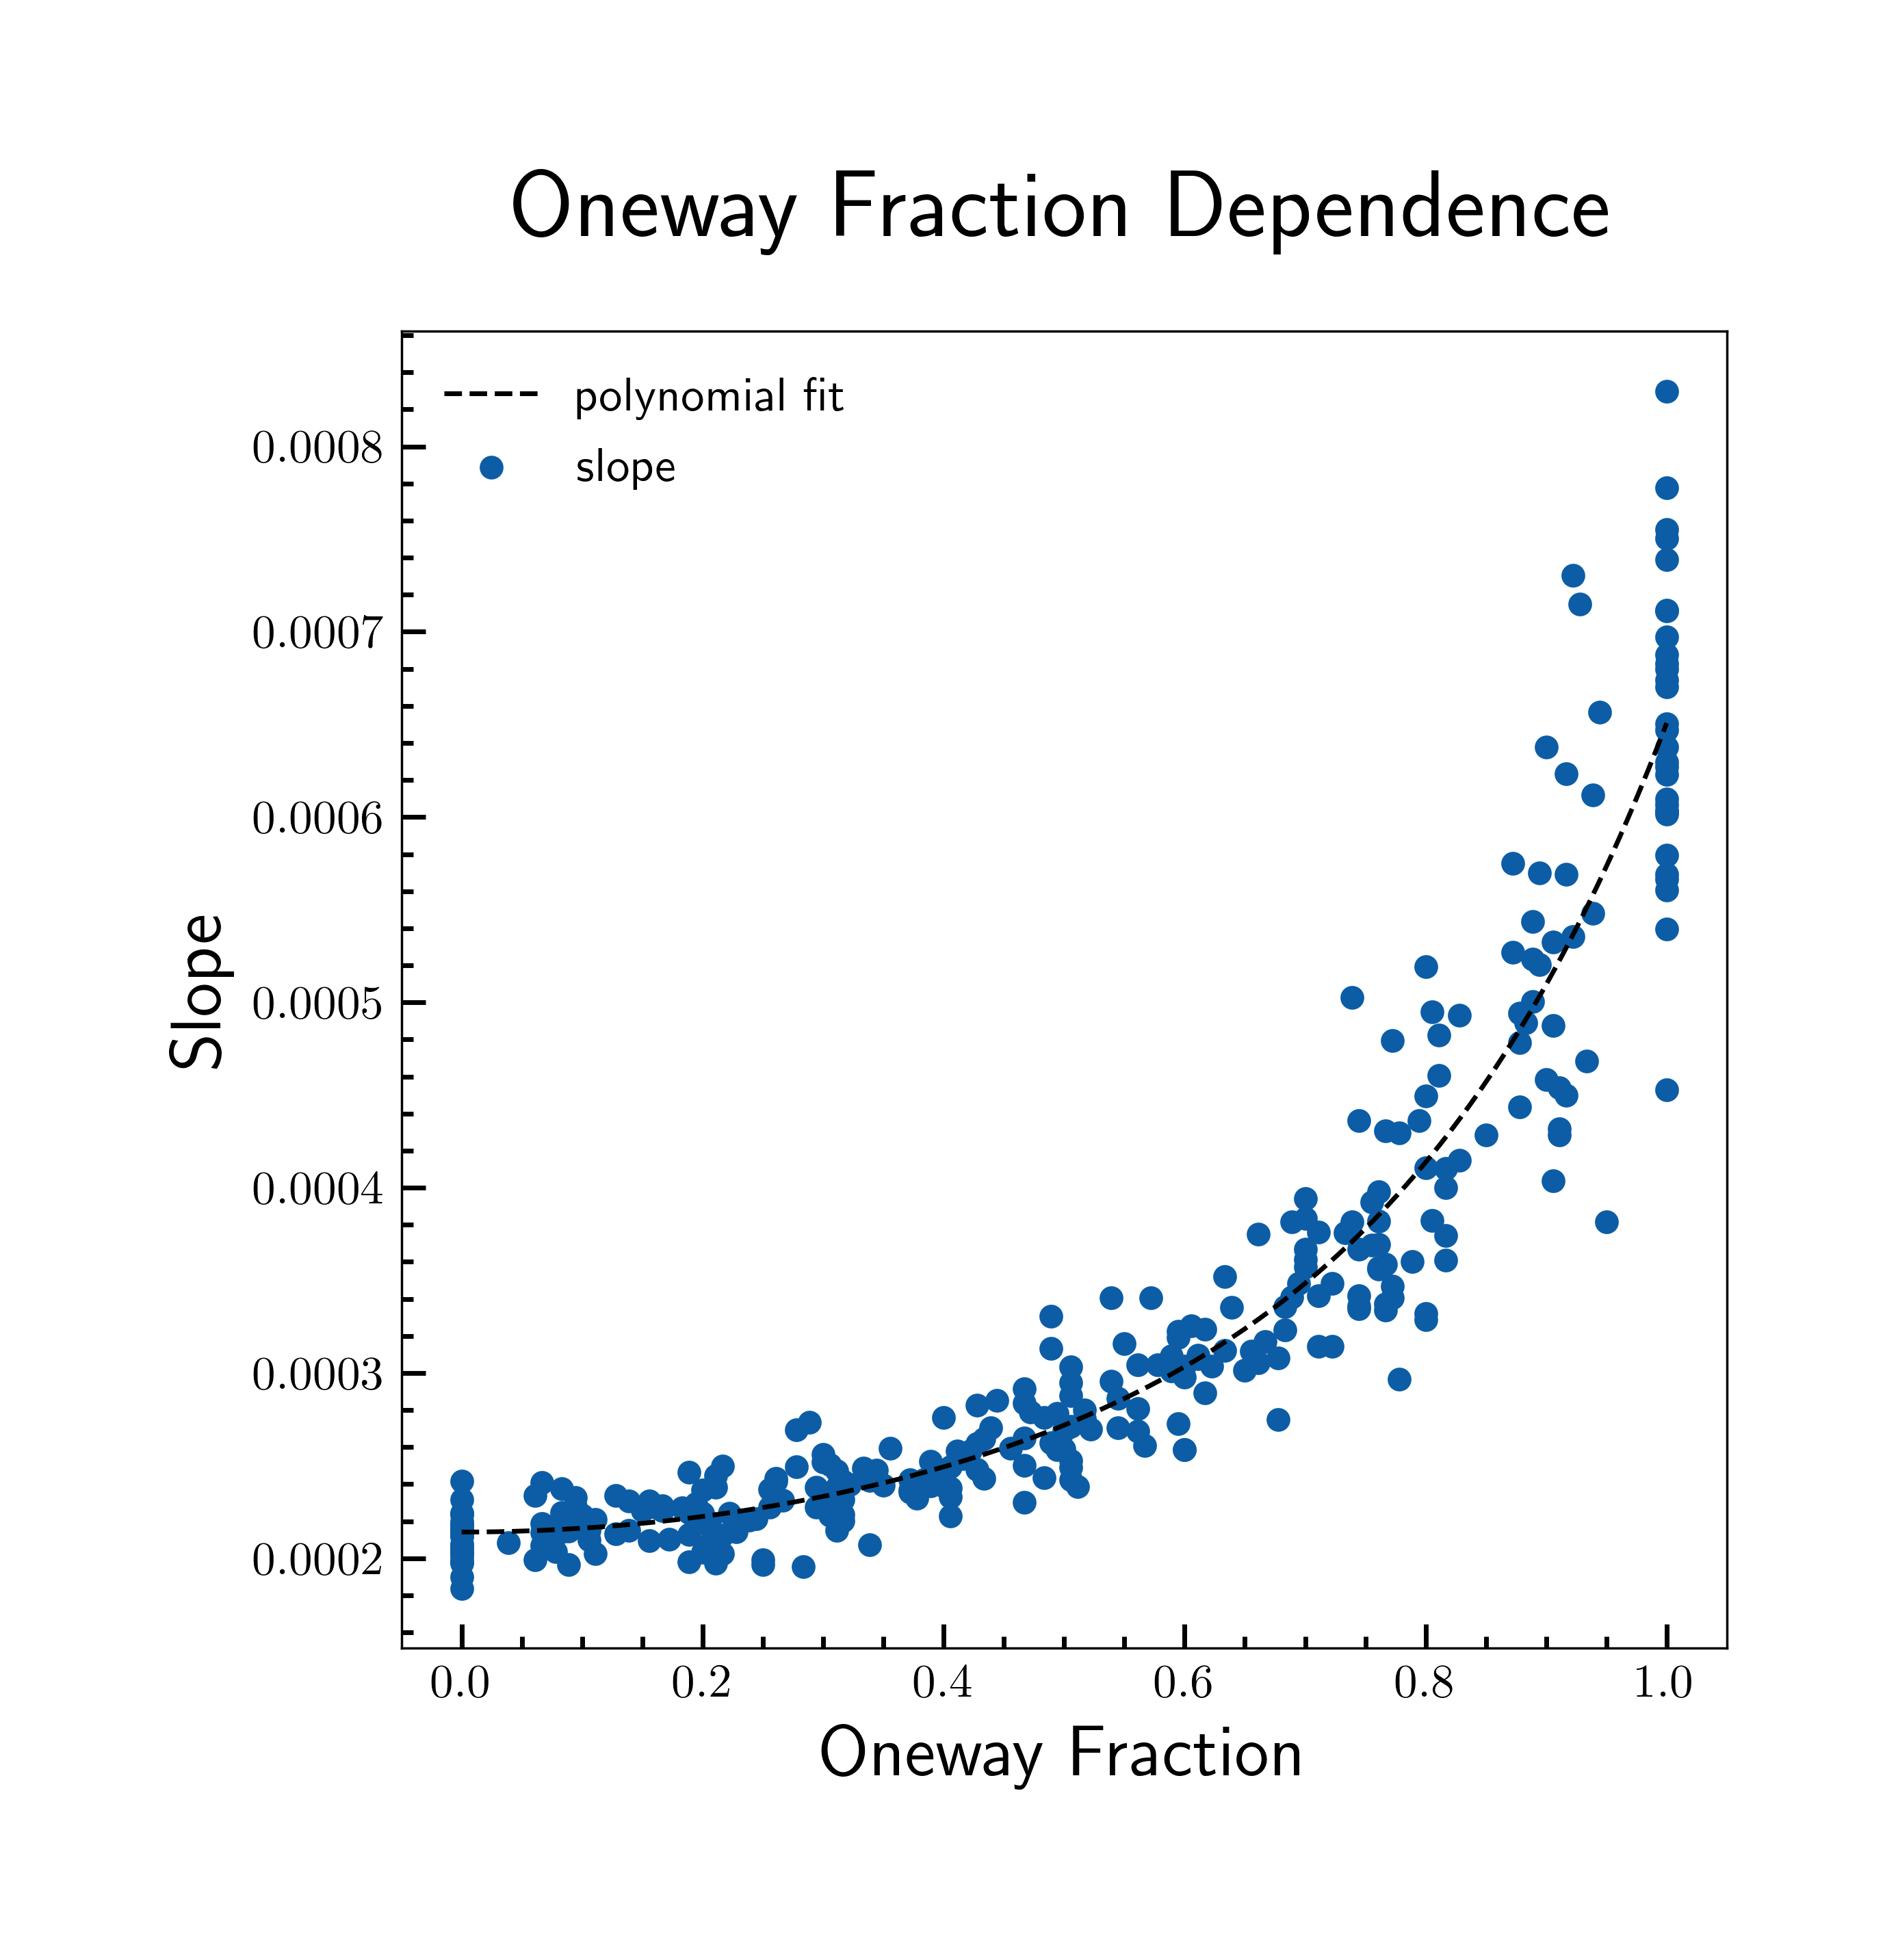
\includegraphics[width=8cm, height=8cm]{oneway_fraction_dependence.png}
                \caption{Variazione della pendenza della retta in funzione della frazione di sensi unici.}
                \label{fig:8}
            \end{minipage}
        \end{figure}

        Si è scelto un range lontano da $car\_number = 1$ dove l'indice di traffico non può seguire un andamento lineare per rispettare il limite ideale.
        Sulla stessa città $10 \times 10$ si sono eseguite varie car increment simulations variando i sensi unici, l'esito è riportato nella figura seguente\footnote{Si è scelto un fit polinomiale per semplicità.}.
        Da tale grafico è evidente che le città con un numero minore di sensi unici rispondono meglio all'aumentare della densità di automobili, come ci dovremmo
        aspettare da un modello di traffico.

        \newpage

        Un'ultima analisi è quella relativa ai tempi di esecuzione della oneway increment simulation su una città $10 \times 10$, il cui esito segue in Fig. \ref{fig:10}.

        \begin{figure}[H]
            \centering
            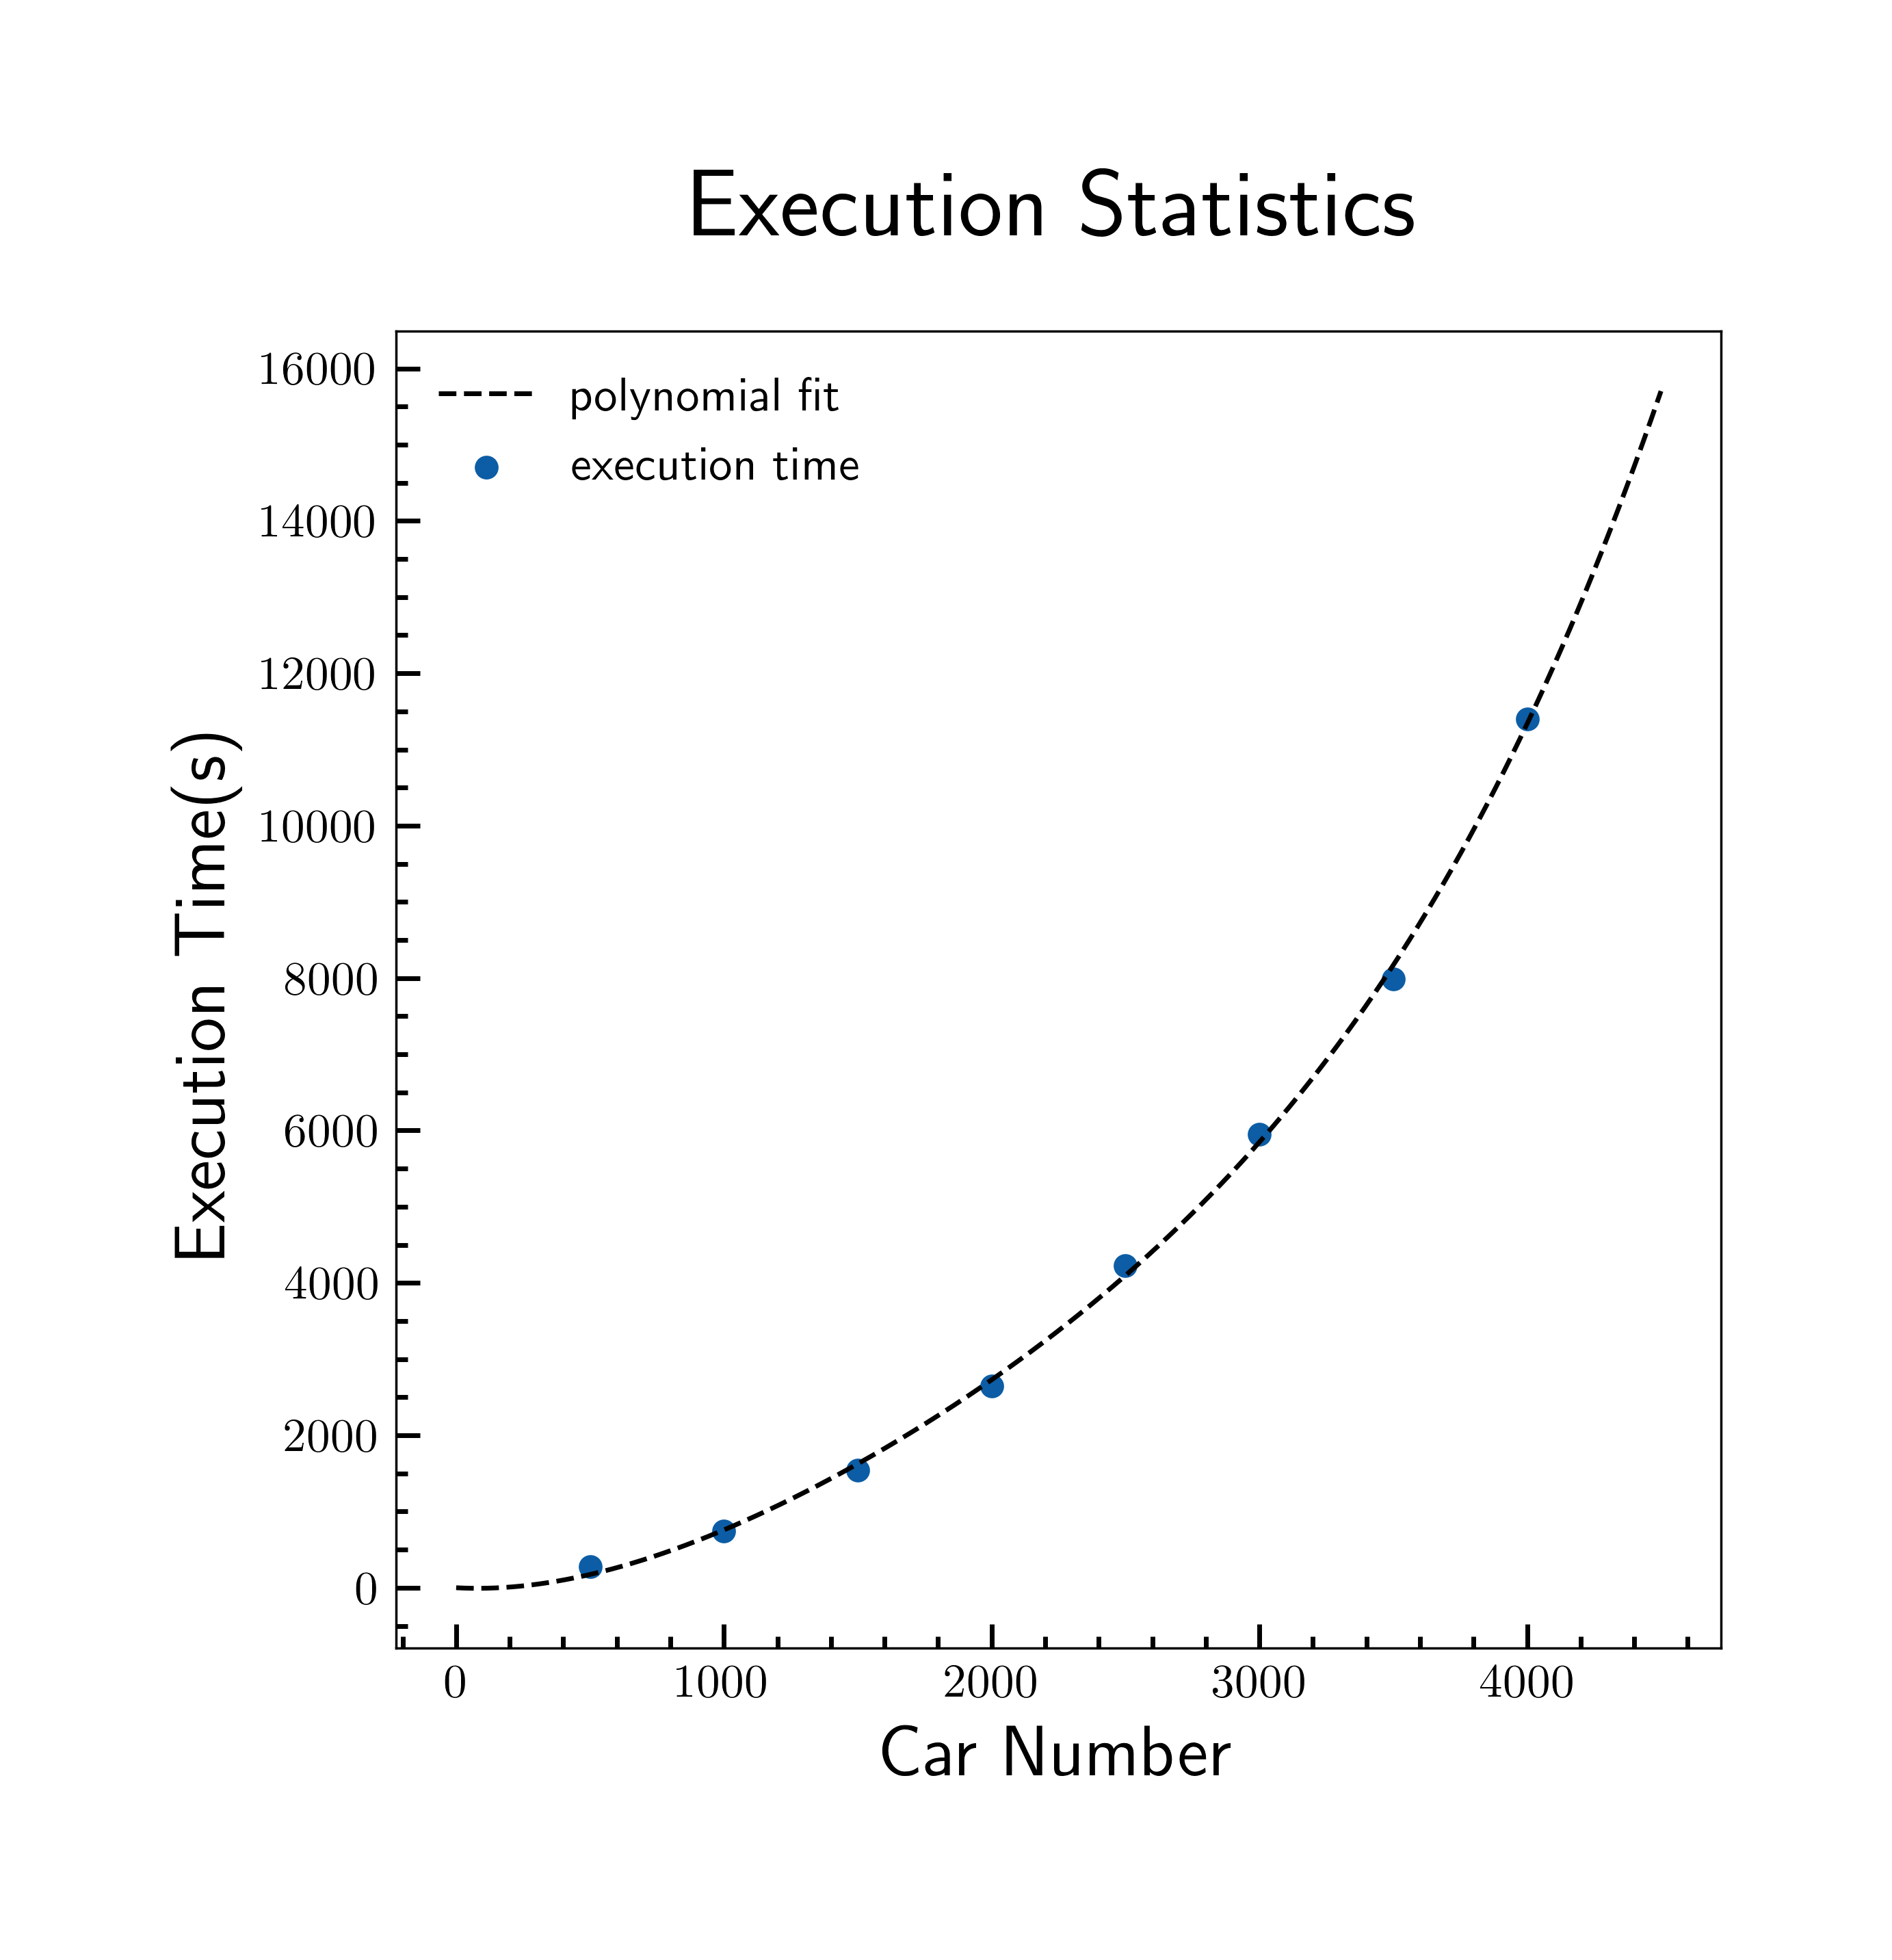
\includegraphics[width=9cm, height=9cm]{execution_time.png}
            \caption{Tempo di esecuzione di oneway increment simulation al variare del numero di auto generate.}
            \label{fig:10}
        \end{figure}

        Tale analisi dà un' idea di come il numero di iterazioni necessarie a portare le auto a destinazione non cresca linearmente come sarebbe in una città ideale,
        e tale effetto è dovuto all'emergere del traffico.\footnote{In realtà è anche dovuto al \ii{sort} chiamato ad ogni iterazione.}

    \subsection{Considerazioni}

        Da tali risultati non possiamo dire che in alcuni casi convenga mettere sensi unici a più corsie piuttosto che sensi alternati,
        tuttavia i risultati suggeriscono l'emergenza del traffico all'aumentare della densità, che è necessario per stabilire la correttezza del 
        nostro modello. Inoltre è verificato il limite ideale, ovvero che per un numero di auto tendente a zero l'indice di traffico tende a 1, e 
        questo ci dà un'ulteriore dato a favore del corretto funzionamento del modello. Gli effetti ricercati possono essere stati nascosti da 
        varie caratteristiche del nostro modello, tali caratteristiche sono discusse nella conclusione.



    
\end{document}